\flushbottom

%% INTRODUCE CONVOLUTION.
%% THE DELTA FUNCTION IS THE LIMIT OF AN AVERAGING FILTER.

%%============================================================================
%%============================================================================
\chapter{The Dirac Delta Function}
\index{Dirac delta function}





I do not know what I appear to the world; but to myself I seem to have been 
only like a boy playing on a seashore, and diverting myself now and then by
finding a smoother pebble or a prettier shell than ordinary, 
whilst the great ocean of truth lay all undiscovered before me.

\begin{flushright}
  - Sir Issac Newton
\end{flushright}





%%=============================================================================
\section{Derivative of the Heaviside Function}
\index{Heaviside function}

The Heaviside function $H(x)$ is defined
\[ 
H(x) =       
\begin{cases}
  0 \quad &\mathrm{for}\ x < 0, \\
  1 \quad &\mathrm{for}\ x > 0.
\end{cases}
\]
%% CONTINUE: Explain why the value at x = 0 doesn't really matter.
The derivative of the Heaviside function is zero for $x \neq 0$.  At $x = 0$
the derivative is undefined.  
We will represent the derivative of the Heaviside function by the Dirac delta
function, $\delta(x)$.  The delta function is zero for $x \neq 0$ and 
infinite at the point $x = 0$.  Since the derivative of $H(x)$ is undefined,
$\delta(x)$ is not a function in the conventional sense of the word.  
One can derive the properties of the delta function rigorously, but the 
treatment in this text will be almost entirely heuristic.


The Dirac delta function is defined by the properties
\[ 
\delta(x) =      
\begin{cases}
  0 \quad &\mathrm{for}\ x \neq 0, \\
  \infty \quad &\mathrm{for}\ x = 0,
\end{cases}
\qquad \mathrm{and} \qquad
\int_{-\infty}^\infty \delta(x)\,\dd x = 1.
\]
The second property comes from the fact that $\delta(x)$ represents the 
derivative of $H(x)$.  
The Dirac delta function is conceptually pictured in Figure~\ref{ddfunction}.


\begin{figure}[h!]
  \begin{center}
    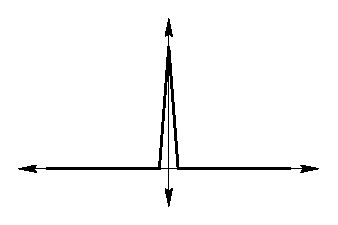
\includegraphics[width=0.3\textwidth]{ode/dirac/ddfunction}
  \end{center}
  \caption{The Dirac delta function.}
  \label{ddfunction}
\end{figure}






Let $f(x)$ be a continuous function that vanishes at infinity.
Consider the integral
\[ 
\int_{-\infty}^\infty f(x) \delta(x)\,\dd x. 
\]
We use integration by parts to evaluate the integral.
\begin{align*}
  \int_{-\infty}^\infty f(x) \delta(x)\,\dd x
  &= \big[ f(x) H(x) \big]_{-\infty}^\infty - \int_{-\infty}^\infty f'(x) H(x)\,\dd x 
  \\
  &= - \int_0^\infty f'(x)\,\dd x 
  \\
  &= [- f(x)]_0^\infty 
  \\
  &= f(0)
\end{align*}

We assumed that $f(x)$ vanishes at infinity in order to use integration
by parts to evaluate the integral.  However, since the delta function is zero
for $x \neq 0$, the integrand is nonzero only at $x = 0$.  Thus the behavior
of the function at infinity should not affect the value of the integral.  
Thus it is reasonable that $f(0) = \int_{-\infty}^\infty f(x)\delta(x)\,\dd x$ holds for
all continuous functions.
By changing variables and noting that $\delta(x)$ is symmetric we can derive 
a more general formula.
\begin{gather*}
  f(0) = \int_{-\infty}^\infty f(\xi) \delta(\xi)\,\dd \xi
  \\
  f(x) = \int_{-\infty}^\infty f(\xi + x) \delta(\xi)\,\dd \xi
  \\
  f(x) = \int_{-\infty}^\infty f(\xi) \delta(\xi - x)\,\dd \xi
  \\
  f(x) = \int_{-\infty}^\infty f(\xi) \delta(x - \xi)\,\dd \xi
\end{gather*}
This formula is very important in solving inhomogeneous differential equations.
%% CONTINUE cite green function



















%%===========================================================================
\section{The Delta Function as a Limit}


Consider a function $b(x,\epsilon)$ defined by
\[ 
b(x,\epsilon) = 
\begin{cases}
  0               &\mathrm{for}\ |x| > \epsilon/2 \\
  \frac{1}{\epsilon} \quad &\mathrm{for}\ |x| < \epsilon/2.
\end{cases}
\]
The graph of $b(x, 1/10)$ is shown in Figure~\ref{epsilon}.

\begin{figure}[h!]
  \begin{center}
    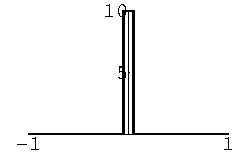
\includegraphics[width=0.3\textwidth]{ode/inhomogeneous/epsilon}
    \caption{Graph of the box function.}
    \label{epsilon}
  \end{center}
\end{figure}


The Dirac delta function $\delta(x)$ can be thought of as $b(x,\epsilon)$ in
the limit as $\epsilon \to 0$. 
Note that the delta function so defined satisfies the properties,
\[ 
\delta(x) = 
\begin{cases}
  0 & \mathrm{for}\ x \neq 0 \\
  \infty & \mathrm{for}\ x = 0
\end{cases}
\qquad \mathrm{and} \qquad
\int_{-\infty}^\infty \delta(x)\,\dd x = 1 
\]



\paragraph{Delayed Limiting Process.}
When the Dirac delta function appears inside an integral, we can think of the
delta function as a delayed limiting process. 
\[ 
\int_{-\infty}^\infty f(x) \delta(x)\,\dd x \equiv \lim_{\epsilon \to 0} \int_{-\infty}^\infty f(x) b(x, \epsilon)\,\dd x. 
\]
Let $f(x)$ be a continuous function and let $F'(x) = f(x)$.  
We compute the integral of $f(x) \delta(x)$.
\begin{align*}
  \int_{-\infty}^\infty f(x) \delta(x)\,\dd x
  &= \lim_{\epsilon \to 0} \frac{1}{\epsilon} \int_{-\epsilon/2}^{\epsilon/2} f(x)\,\dd x 
  \\
  &= \lim_{\epsilon \to 0} \frac{1}{\epsilon} [F(x)]_{-\epsilon/2}^{\epsilon/2} 
  \\
  &= \lim_{\epsilon \to 0} \frac{F(\epsilon/2) - F(-\epsilon/2)}{\epsilon} 
  \\
  &= F'(0) 
  \\
  &= f(0)
\end{align*}











%%===========================================================================
\section{Higher Dimensions}






We can define a Dirac delta function in $n$-dimensional Cartesian space, 
$\delta_n(\mathbf{x})$, $\mathbf{x} \in \mathbb{R}^n$.
It is defined by the following two properties.
\begin{gather*}
  \delta_n(\mathbf{x}) = 0 
  \quad \mathrm{for} \quad \mathbf{x} \neq \mathbf{0}
  \\
  \int_{\mathbb{R}^n} \delta_n(\mathbf{x}) \,\dd \mathbf{x} = 1
\end{gather*}
It is easy to verify, that the $n$-dimensional Dirac delta function can be 
written as a product of $1$-dimensional Dirac delta functions.
\[
\delta_n(\mathbf{x}) = \prod_{k=1}^n \delta(x_k)
\]





%%===========================================================================
\section{Non-Rectangular Coordinate Systems}




We can derive Dirac delta functions in non-rectangular coordinate systems
by making a change of variables in the relation,
\[
\int_{\mathbb{R}^n} \delta_n(\mathbf{x}) \,\dd \mathbf{x} = 1
\]
Where the transformation is non-singular, one merely divides the Dirac 
delta function by the Jacobian of the transformation to the coordinate system.




\begin{Example}
  Consider the Dirac delta function in cylindrical coordinates, $(r, \theta, z)$.
  The Jacobian is $J = r$.
  \[
  \int_{-\infty}^\infty \int_0^{2 \pi} \int_0^\infty \delta_3 \left( \mathbf{x} - \mathbf{x}_0 \right) 
  r \,\dd r \,\dd \theta \,\dd z = 1
  \]
  For $r_0 \neq 0$, the Dirac Delta function is
  \[
  \delta_3 \left( \mathbf{x} - \mathbf{x}_0 \right) 
  = \frac{1}{r} \delta \left( r - r_0 \right) \delta \left( \theta - \theta_0 \right)
  \delta \left( z - z_0 \right)
  \]
  since it satisfies the two defining properties.
  \[
  \frac{1}{r} \delta \left( r - r_0 \right) \delta \left( \theta - \theta_0 \right)
  \delta \left( z - z_0 \right) = 0 
  \quad \mathrm{for} \quad ( r, \theta, z ) \neq \left( r_0, \theta_0, z_0 \right)
  \]
  \begin{multline*}
    \int_{-\infty}^\infty \int_0^{2 \pi} \int_0^\infty \frac{1}{r} \delta \left( r - r_0 \right) \delta \left( \theta - \theta_0 \right)
    \delta \left( z - z_0 \right) r \,\dd r \,\dd \theta \,\dd z
    \\
    = \int_0^\infty \delta \left( r - r_0 \right) \,\dd r 
    \int_0^{2 \pi} \delta \left( \theta - \theta_0 \right) \,\dd \theta 
    \int_{-\infty}^\infty \delta \left( z - z_0 \right) \,\dd z = 1
  \end{multline*}
  For $r_0 = 0$, we have
  \[
  \delta_3 \left( \mathbf{x} - \mathbf{x}_0 \right) 
  = \frac{1}{2 \pi r} \delta \left( r \right) \delta \left( z - z_0 \right)
  \]
  since this again satisfies the two defining properties.
  \begin{gather*}
    \frac{1}{2 \pi r} \delta \left( r \right)
    \delta \left( z - z_0 \right) = 0 
    \quad \mathrm{for} \quad ( r, z ) \neq \left( 0, z_0 \right)
    \\
    \int_{-\infty}^\infty \int_0^{2 \pi} \int_0^\infty \frac{1}{2 \pi r} \delta \left( r \right) 
    \delta \left( z - z_0 \right) r \,\dd r \,\dd \theta \,\dd z
    = \frac{1}{2 \pi} \int_0^\infty \delta \left( r \right) \,\dd r 
    \int_0^{2 \pi} \,\dd \theta 
    \int_{-\infty}^\infty \delta \left( z - z_0 \right) \,\dd z = 1
  \end{gather*}
\end{Example}












\raggedbottom
%%===========================================================================
\exercises{
\pagebreak
\flushbottom
\section{Exercises}





\begin{Exercise}
  \label{exercise f0-f0+2=intfd}
  Let $f(x)$ be a function that is continuous except for a jump discontinuity
  at $x = 0$.  Using a delayed limiting process, show that
  \[ 
  \frac{f(0^-) + f(0^+)}{2} = \int_{-\infty}^\infty f(x)\delta(x)\,\dd x.
  \]

  \hintsolution{f0-f0+2=intfd}
\end{Exercise}



\begin{Exercise}
  \label{exercise ode dirac symmetric}
  Show that the Dirac delta function is symmetric.
  \[ 
  \delta(- x) = \delta(x)
  \]

  \hintsolution{ode dirac symmetric}
\end{Exercise}




\begin{Exercise}
  \label{exercise d(cx)=d(x)/c}
  Show that
  \[ 
  \delta(c x) = \frac{\delta(x)}{|c|}.
  \]

  \hintsolution{d(cx)=d(x)/c}
\end{Exercise}







\begin{Exercise}
  \label{exercise dcx=1cdx}
  We will consider the Dirac delta function with a function as on argument,
  $\delta(y(x))$.  Assume that $y(x)$ has simple zeros at the points $\{ x_n \}$.
  \[
  y(x_n) = 0, \quad y'(x_n) \neq 0
  \]
  Further assume that $y(x)$ has no multiple zeros.  (If $y(x)$ has multiple
  zeros $\delta(y(x))$ is not well-defined in the same sense that $1/0$ is not 
  well-defined.)
  Prove that 
  \[
  \delta(y(x)) = \sum_n \frac{\delta(x - x_n)}{|y'(x_n)|}.
  \]
  
  \hintsolution{dcx=1cdx}
\end{Exercise}







\begin{Exercise}
  \label{exercise ode dirac dnx}
  Justify the identity
  \[
  \int_{-\infty}^\infty f(x) \delta^{(n)}(x) \,\dd x = (-1)^n f^{(n)}(0)
  \]
  From this show that
  \[
  \delta^{(n)}(-x) = (-1)^n \delta^{(n)}(x)
  \quad \mathrm{and} \quad
  x \delta^{(n)}(x) = - n \delta^{(n-1)}(x).
  \]

  \hintsolution{ode dirac dnx}
\end{Exercise}









\begin{Exercise}
  \label{exercise ode dirac nd jacobian}
  Consider $\mathbf{x} = (x_1, \ldots, x_n) \in \mathbb{R}^n$ and the curvilinear
  coordinate system $\boldsymbol{\xi} = (\xi_1, \ldots, \xi_n)$.
  Show that
  \[
  \delta(\mathbf{x} - \mathbf{a}) = \frac{ \delta(\boldsymbol{\xi} - \boldsymbol{\alpha}) }{ |J| }
  \]
  where $\mathbf{a}$ and $\boldsymbol{\alpha}$ are corresponding points in the two 
  coordinate systems and $J$ is the Jacobian of the transformation
  from $\mathbf{x}$ to $\boldsymbol{\xi}$.
  \[
  J \equiv \frac{\partial \mathbf{x}}{\partial \boldsymbol{\xi}}
  \]

  \hintsolution{ode dirac nd jacobian}
\end{Exercise}






\begin{Exercise}
  \label{exercise dirac delta spherical}
  Determine the Dirac delta function in spherical coordinates, 
  $(r, \theta, \phi)$.
  \[
  x = r \cos \theta \sin \phi, \qquad
  y = r \sin \theta \sin \phi, \qquad
  z = r \cos \phi
  \]

  \hintsolution{dirac delta spherical}
\end{Exercise}














\raggedbottom
}
%%============================================================================
\hints{
\pagebreak
\flushbottom
\section{Hints}



\begin{Hint}
  \label{hint f0-f0+2=intfd}
  %% CONTINUE
\end{Hint}


\begin{Hint}
  \label{hint ode dirac symmetric}
  Verify that $\delta(-x)$ satisfies the two properties of the Dirac 
  delta function.
\end{Hint}



\begin{Hint}
  \label{hint d(cx)=d(x)/c}
  Evaluate the integral,
  \[
  \int_{-\infty}^\infty f(x) \delta(c x)\,\dd x,
  \]
  by noting that the Dirac delta function is symmetric
  and making a change of variables.
\end{Hint}



\begin{Hint}
  \label{hint dcx=1cdx}
  Let the points $\{ \xi_m \}$ partition the interval $(-\infty \ldots \infty)$ such that $y'(x)$
  is monotone on each interval $(\xi_m \ldots \xi_{m+1})$.  Consider some such interval,
  $(a \ldots b) \equiv (\xi_m \ldots \xi_{m+1})$.  Show that
  \[
  \int_a^b \delta(y(x))\,\dd x
  = \begin{cases}
    \int_\alpha^\beta \frac{\delta(y)}{|y'(x_n)|}\,\dd y &\mathrm{if}\ y(x_n) = 0\ 
    \mathrm{for}\ a < x_n < b \\
    0 &\mathrm{otherwise}
  \end{cases}
  \]
  for $\alpha = \min(y(a),y(b))$ and $\beta = \max(y(a),y(b))$.
  Now consider the integral on the interval $(-\infty \ldots \infty)$ as the sum of 
  integrals on the intervals $\{ (\xi_m \ldots \xi_{m+1}) \}$.
\end{Hint}




\begin{Hint}
  \label{hint ode dirac dnx}
  Justify the identity,
  \[
  \int_{-\infty}^\infty f(x) \delta^{(n)}(x) \,\dd x = (-1)^n f^{(n)}(0),
  \]
  with integration by parts.
  %% CONTINUE
\end{Hint}




\begin{Hint}
  \label{hint ode dirac nd jacobian}
  The Dirac delta function is defined by the following two properties.
  \begin{gather*}
    \delta(\mathbf{x} - \mathbf{a}) = 0 
    \quad \mathrm{for} \quad \mathbf{x} \neq \mathbf{a}
    \\
    \int_{\mathbb{R}^n} \delta(\mathbf{x} - \mathbf{a}) \,\dd \mathbf{x} = 1
  \end{gather*}
  Verify that $\delta(\boldsymbol{\xi} - \boldsymbol{\alpha}) / |J|$ satisfies these properties
  in the $\boldsymbol{\xi}$ coordinate system.
\end{Hint}





\begin{Hint}
  \label{hint dirac delta spherical}
  Consider the special cases $\phi_0 = 0,\pi$ and $r_0 = 0$.
\end{Hint}









\raggedbottom
}
%%============================================================================
\solutions{
\pagebreak
\flushbottom
\section{Solutions}








\begin{Solution}
  \label{solution f0-f0+2=intfd}
  Let $F'(x) = f(x)$.
  \begin{align*}
    \int_{-\infty}^\infty f(x)\delta(x)\,\dd x
    &= \lim_{\epsilon \to 0} \frac{1}{\epsilon} \int_{-\infty}^\infty f(x) b(x,\epsilon)\,\dd x 
    \\
    &= \lim_{\epsilon \to 0} \frac{1}{\epsilon} \left( \int_{-\epsilon/2}^0 f(x) b(x, \epsilon)\,\dd x 
      + \int_0^{\epsilon/2} f(x) b(x, \epsilon)\,\dd x \right) 
    \\
    &= \lim_{\epsilon \to 0} \frac{1}{\epsilon} \left( (F(0) - F(-\epsilon/2)) + (F(\epsilon/2) - F(0)) \right) 
    \\
    &= \lim_{\epsilon \to 0} \frac{1}{2} \left( \frac{F(0) - F(-\epsilon/2)}{\epsilon/2}
      + \frac{F(\epsilon/2) - F(0)}{\epsilon/2} \right) 
    \\
    &= \frac{F'(0^-) + F'(0^+)}{2} 
    \\
    &= \frac{f(0^-) + f(0^+)}{2}
  \end{align*}
\end{Solution}





\begin{Solution}
  \label{solution ode dirac symmetric}
  $\delta(-x)$ satisfies the two properties of the Dirac delta function.
  \begin{gather*}
    \delta(-x) = 0\ \mathrm{for}\ x \neq 0
    \\
    \int_{-\infty}^\infty \delta(-x)\,\dd x = \int_\infty^{-\infty} \delta(x) \,(-\dd x) = \int_{-\infty}^\infty \delta(-x)\,\dd x = 1
  \end{gather*}
  Therefore $\delta(-x) = \delta(x)$.
\end{Solution}






\begin{Solution}
  \label{solution d(cx)=d(x)/c}
  We note the the Dirac delta function is symmetric and we make a change of
  variables to derive the identity.
  \begin{align*}
    \int_{-\infty}^\infty \delta(c x)\,\dd x 
    &= \int_{-\infty}^\infty \delta(|c| x)\,\dd x 
    \\
    &= \int_{-\infty}^\infty \frac{\delta(x)}{|c|}\,\dd x 
  \end{align*}
  \[ 
  \boxed{
    \delta(c x) = \frac{\delta(x)}{|c|}
    }
  \]
\end{Solution}







\begin{Solution}
  \label{solution dcx=1cdx}
  Let the points $\{ \xi_m \}$ partition the interval $(-\infty \ldots \infty)$ such that $y'(x)$
  is monotone on each interval $(\xi_m \ldots \xi_{m+1})$.  Consider some such interval,
  $(a \ldots b) \equiv (\xi_m \ldots \xi_{m+1})$.  Note that $y'(x)$ is either 
  entirely positive or entirely negative in the interval.  First consider 
  the case when it is positive.  In this case $y(a) < y(b)$.
  \begin{align*}
    \int_a^b \delta(y(x))\,\dd x
    &= \int_{y(a)}^{y(b)} \delta(y) \left( \frac{\dd y}{\dd x} \right)^{-1} \,\dd y 
    \\
    &= \int_{y(a)}^{y(b)} \frac{\delta(y)}{y'(x)}\,\dd y 
    \\
    &= \begin{cases}
      \int_{y(a)}^{y(b)} \frac{\delta(y)}{y'(x_n)}\,\dd y &\mathrm{for}\ y(x_n) = 0\ 
      \mathrm{if}\ y(a) < 0 < y(b) \\
      0 &\mathrm{otherwise}
    \end{cases}
  \end{align*}
  Now consider the case that $y'(x)$ is negative on the interval so 
  $y(a) > y(b)$.
  \begin{align*}
    \int_a^b \delta(y(x))\,\dd x
    &= \int_{y(a)}^{y(b)} \delta(y) \left( \frac{\dd y}{\dd x} \right)^{-1} \,\dd y 
    \\
    &= \int_{y(a)}^{y(b)} \frac{\delta(y)}{y'(x)}\,\dd y 
    \\
    &= \int_{y(b)}^{y(a)} \frac{\delta(y)}{-y'(x)}\,\dd y 
    \\
    &= \begin{cases}
      \int_{y(b)}^{y(a)} \frac{\delta(y)}{-y'(x_n)}\,\dd y &\mathrm{for}\ y(x_n) = 0\ 
      \mathrm{if}\ y(b) < 0 < y(a) \\
      0 &\mathrm{otherwise}
    \end{cases}
  \end{align*}
  We conclude that
  \[
  \int_a^b \delta(y(x))\,\dd x
  = \begin{cases}
    \int_\alpha^\beta \frac{\delta(y)}{|y'(x_n)|}\,\dd y &\mathrm{if}\ y(x_n) = 0\ 
    \mathrm{for}\ a < x_n < b \\
    0 &\mathrm{otherwise}
  \end{cases}
  \]
  for $\alpha = \min(y(a),y(b))$ and $\beta = \max(y(a),y(b))$.

  Now we turn to the integral of $\delta(y(x))$ on $(-\infty \ldots \infty)$.
  Let $\alpha_m = \min(y(\xi_m),y(\xi_m))$ and $\beta_m = \max(y(\xi_m),y(\xi_m))$.
  \begin{align*}
    \int_{-\infty}^\infty \delta(y(x))\,\dd x
    &= \sum_m \int_{\xi_m}^{\xi_{m+1}} \delta(y(x))\,\dd x
    \\
    &= \sum_{\substack{m\\x_n \in (\xi_m \ldots \xi_{m+1})}} \int_{\xi_m}^{\xi_{m+1}} \delta(y(x))\,\dd x
    \\
    &= \sum_{\substack{m\\x_n \in (\xi_m \ldots \xi_{m+1})}} 
    \int_{\alpha_m}^{\beta_{m+1}} \frac{\delta(y)}{|y'(x_n)|}\,\dd y
    \\
    &= \sum_n \int_{-\infty}^\infty \frac{\delta(y)}{|y'(x_n)|}\,\dd y
    \\
    &= \int_{-\infty}^\infty \sum_n \frac{\delta(y)}{|y'(x_n)|}\,\dd y
  \end{align*}
  \[
  \boxed{
    \delta(y(x)) = \sum_n \frac{\delta(x - x_n)}{|y'(x_n)|}
    }
  \]
\end{Solution}






\begin{Solution}
  \label{solution ode dirac dnx}
  To justify the identity,
  \[
  \int_{-\infty}^\infty f(x) \delta^{(n)}(x) \,\dd x = (-1)^n f^{(n)}(0),
  \]
  we will use integration by parts.
  \begin{align*}
    \int_{-\infty}^\infty f(x) \delta^{(n)}(x) \,\dd x
    &= \left[ f(x) \delta^{(n-1)}(x) \right]_{-\infty}^\infty - \int_{-\infty}^\infty f'(x) \delta^{(n-1)}(x) \,\dd x
    \\
    &= - \int_{-\infty}^\infty f'(x) \delta^{(n-1)}(x) \,\dd x
    \\
    &= (-1)^n \int_{-\infty}^\infty f^{(n)}(x) \delta(x) \,\dd x
    \\
    &= (-1)^n f^{(n)}(0)
  \end{align*}

  CONTINUE HERE
  \[
  \delta^{(n)}(-x) = (-1)^n \delta^{(n)}(x)
  \quad \mathrm{and} \quad
  x \delta^{(n)}(x) = - n \delta^{(n-1)}(x).
  \]
\end{Solution}








\begin{Solution}
  \label{solution ode dirac nd jacobian}
  The Dirac delta function is defined by the following two properties.
  \begin{gather*}
    \delta(\mathbf{x} - \mathbf{a}) = 0 
    \quad \mathrm{for} \quad \mathbf{x} \neq \mathbf{a}
    \\
    \int_{\mathbb{R}^n} \delta(\mathbf{x} - \mathbf{a}) \,\dd \mathbf{x} = 1
  \end{gather*}
  We verify that $\delta(\boldsymbol{\xi} - \boldsymbol{\alpha}) / |J|$ satisfies these properties
  in the $\boldsymbol{\xi}$ coordinate system.
  \begin{align*}
    \frac{ \delta(\boldsymbol{\xi} - \boldsymbol{\alpha}) }{ |J| }
    &= \frac{ \delta(\xi_1 - \alpha_1) \cdots \delta(\xi_n - \alpha_n) }{ |J| }
    \\
    &= 0 \quad \mathrm{for} \quad \boldsymbol{\xi} \neq \boldsymbol{\alpha}
  \end{align*}
  \begin{align*}
    \int \frac{ \delta(\boldsymbol{\xi} - \boldsymbol{\alpha}) }{ |J| }|J|\,\dd \boldsymbol{\xi}
    &= \int \delta(\boldsymbol{\xi} - \boldsymbol{\alpha}) \,\dd \boldsymbol{\xi}
    \\
    &= \int \delta(\xi_1 - \alpha_1) \cdots \delta(\xi_n - \alpha_n) \,\dd \boldsymbol{\xi}
    \\
    &= \int \delta(\xi_1 - \alpha_1)\,\dd \xi_1 \cdots \int \delta(\xi_n - \alpha_n)\,\dd \xi_n
    \\
    &= 1
  \end{align*}
  We conclude that $\delta(\boldsymbol{\xi} - \boldsymbol{\alpha}) / |J|$ is the Dirac delta function
  in the $\boldsymbol{\xi}$ coordinate system.
  \[
  \delta(\mathbf{x} - \mathbf{a}) = \frac{ \delta(\boldsymbol{\xi} - \boldsymbol{\alpha}) }{ |J| }
  \]
\end{Solution}






\begin{Solution}
  \label{solution dirac delta spherical}
  We consider the Dirac delta function in spherical coordinates, $(r, \theta, \phi)$.
  The Jacobian is $J = r^2 \sin(\phi)$.
  \[
  \int_0^\pi \int_0^{2 \pi} \int_0^\infty \delta_3 \left( \mathbf{x} - \mathbf{x}_0 \right) 
  r^2 \sin(\phi) \,\dd r \,\dd \theta \,\dd \phi = 1
  \]
  For $r_0 \neq 0$, and $\phi_0 \neq 0,\pi$, the Dirac Delta function is
  \[
  \delta_3 \left( \mathbf{x} - \mathbf{x}_0 \right) 
  = \frac{1}{r^2 \sin(\phi)} \delta \left( r - r_0 \right) \delta \left( \theta - \theta_0 \right)
  \delta \left( \phi - \phi_0 \right)
  \]
  since it satisfies the two defining properties.
  \[
  \frac{1}{r^2 \sin(\phi)} \delta \left( r - r_0 \right) \delta \left( \theta - \theta_0 \right)
  \delta \left( \phi - \phi_0 \right) = 0 
  \quad \mathrm{for} \quad ( r, \theta, \phi ) \neq \left( r_0, \theta_0, \phi_0 \right)
  \]
  \begin{multline*}
    \int_0^\pi \int_0^{2 \pi} \int_0^\infty \frac{1}{r^2 \sin(\phi)} 
    \delta \left( r - r_0 \right) \delta \left( \theta - \theta_0 \right) \delta \left( \phi - \phi_0 \right)
    r^2 \sin(\phi) \,\dd r \,\dd \theta \,\dd \phi
    \\
    = \int_0^\infty \delta \left( r - r_0 \right) \,\dd r 
    \int_0^{2 \pi} \delta \left( \theta - \theta_0 \right) \,\dd \theta 
    \int_0^\pi \delta \left( \phi - \phi_0 \right) \,\dd \phi = 1
  \end{multline*}
  For $\phi_0 = 0$ or $\phi_0 = \pi$, the Dirac delta function is
  \[
  \delta_3 \left( \mathbf{x} - \mathbf{x}_0 \right) 
  = \frac{1}{2 \pi r^2 \sin(\phi)} \delta \left( r - r_0 \right) \delta \left( \phi - \phi_0 \right).
  \]
  We check that the value of the integral is unity.
  \begin{multline*}
    \int_0^\pi \int_0^{2 \pi} \int_0^\infty \frac{1}{2 \pi r^2 \sin(\phi)} 
    \delta \left( r - r_0 \right) \delta \left( \phi - \phi_0 \right)
    r^2 \sin(\phi) \,\dd r \,\dd \theta \,\dd \phi
    \\
    = \frac{1}{2 \pi} \int_0^\infty \delta \left( r - r_0 \right) \,\dd r 
    \int_0^{2 \pi} \,\dd \theta 
    \int_0^\pi \delta \left( \phi - \phi_0 \right) \,\dd \phi = 1
  \end{multline*}
  For $r_0 = 0$ the Dirac delta function is
  \[
  \delta_3 \left( \mathbf{x} \right) 
  = \frac{1}{4 \pi r^2} \delta \left( r \right)
  \]
  We verify that the value of the integral is unity.
  \[
  \int_0^\pi \int_0^{2 \pi} \int_0^\infty \frac{1}{4 \pi r^2} 
  \delta \left( r - r_0 \right) r^2 \sin(\phi) \,\dd r \,\dd \theta \,\dd \phi
  = \frac{1}{4 \pi} \int_0^\infty \delta \left( r \right) \,\dd r 
  \int_0^{2 \pi} \,\dd \theta 
  \int_0^\pi \sin(\phi) \,\dd \phi = 1
  \]
\end{Solution}












\raggedbottom
}
